\section{Методы}
%\chapter{Методы}

Наилучшие результаты в большинстве задач обработки изображений достигаются с использованием нейронных сетей.
Нейросеть $f$~--- это отображение из некоторого параметризованного класса 
\begin{equation}
    \mathcal{F} = \{f_\theta \colon \mathcal{X} \mapsto \mathcal{Y}, \theta \in \Theta \subset \mathbb{R}^D\}.
\end{equation}

Очень часто нейросеть можно представить в виде суперпозиции отображений
$f = h \circ g, \; g \colon \mathcal{X} \mapsto \mathcal{Z}, \; h\colon \mathcal{Z} \mapsto \mathcal{Y}$.
Иными словами, объект $x$ сперва преобразовывается в некоторое промежуточное (латентное, скрытое) представление $z = g(x)$,
а затем уже по скрытому представлению $z$ делается предсказание $\hat{y} = h(z)$.
Таким образом, отображение $g$ осуществляет преобразование признакового пространства.
В англоязычной литературе функцию $g$ обычно называют <<feature extractor>> или <<encoder>>.
Функцию $h$ называют <<head>> или <<decoder>>.

Сегментация с учителем может рассматриваться как классификация пикселей.
В таком случае объекты $x \in \mathcal{X}$ --- это векторные представления пикселей.
Для каждого пикселя $x$ строится его латентное представление $z = h(x)$, из которого decoder предсказывает семантический класс.
Как отсюда перейти к unsupervised-сценарию? 

Аналог классификации в режиме без учителя --- это кластеризация.
Если мы можем обучить encoder без доступа к меткам так, чтобы представления пикселей образовывали семантические кластера,
то можно заменить decoder на стандартный метод кластеризации (скажем, KMeans).
По существу, на этом и основано большинство методов сегментации без учителя,
и их отличия заключаются в том, каким образом обучается encoder.

Иногда у нас всё-таки есть небольшое количество размеченных изображений, и хочется их использовать.
Поэтому интересно рассматривать также и методы Few-Shot сегментации.
В них, как правило, тоже сначала обучается encoder без доступа к меткам (стадия \textit{предобучения}), а потом происходит 
\textit{дообучение} на имеющихся изображениях (либо всей сети $f = h \circ g$, либо обучается только лёгкий decoder $h$).
На самом деле, предобученный encoder часто можно использовать для разных задач~--- детекции, image retrieval, copy detection и другие.
На практике это часто является преимуществом, поэтому я буду упоминать об этом, говоря о методах, которые это позволяют.
\bigskip

Итак, вопрос сводится к тому, что надо придумать способ предобучения encoder-а, который не требует вручную размеченных данных.
Давайте посмотрим, какие существуют решения.
\subsection{IIC}
    \textit{В одно предложение: максимизация взаимной информации между предсказаниями сегментации для двух версий одного изображения.}
    \bigskip

    Б\'{о}льшая часть алгоритмов сегментации без учителя на момент написания этой статьи базировалась на попытке 
    использовать нейронные сети и классические алгоритмы кластеризации.
    Такие решения страдали от нестабильного обучения и вырожденных решений~--- 
    когда всё обьединялось в один кластер, или в какие-то кластера не попадало ни одной точки.
    Авторы статьи Invariant Information Clustering предложили новую функцию потерь, 
    которая естественным образом позволила избежать проблемы вырожденности.
    Этот подход также позволил хорошо решить задачу кластеризации изображений.

    \subsubsection{Функция потерь}
    Пусть $x, x' \in \mathcal{X}$~--- это пара из совместного распределения $\mathcal{P}(x, x')$.
    Например, это могут быть разные изображения одного объекта.
    Цель IIC~--- выучить encoder $\Phi\colon \mathcal{X} \mapsto \mathcal{Y}$, который будет сохранять в 
    латентном представлении $z = \Phi(x)$ существенные особенности объекта и отбрасывать незначительные детали.
    Это формализуется с использованием понятия взаимной информации:
    \begin{equation}
        \Phi^* = \argmax_{\Phi} I \left( \Phi(x), \Phi(x') \right)
    \end{equation}

    В процессе решения такой задачи оптимизации представления $z = \Phi(x), z' = \Phi(x')$ становятся всё ближе друг к другу.
    Однако, в отличии от методов, основанных на KMeans, здесь не появляется вырождённых решений,
    так как взаимная информация включает в себя безусловную и условную энтропию. А именно, 
    \begin{equation}
        I(z, z') = H(z) - H(z\, | \, z')
    \end{equation}
    Максимальное значение для $H(z)$ равно $\ln C$, где $C$~--- число кластеров. Оно достигается, когда все кластеры равновероятны.
    Минимальное значение $H(z \, | \, z')$~--- $0$, достигается, когда $z$ идеально восстанавливается по $z'$.
    Таким образом, значение взаимной информации не будет максимальным, если всё принадлежит одному кластеру.
    Можно рассматривать безусловную энтропию как регуляризацию.

    Важно отметить, что отображение $\Phi$ должно иметь ограниченную выразительность.
    В противном случае задача максимизации решается тривиально~--- достаточно положить $\Phi(x) = x$.
    Часто можно избежать этого снижением размерности латентного пространства $\mathcal{Z}$.
    В случае кластеризации пикселей есть также и другой способ: на выходе для каждого пикселя мы ожидаем один из классов $y \in \mathcal{Y} = \{1, \ldots, C\}$.
    Авторы рассматривают нечёткую кластеризацию, поэтому для каждого пикселя его представление~--- это дискретное распределение по $C$ кластерам.
    $k$-я компонента интерпретируется как оценка вероятности принадлежности кластеру с номером $k$: $\mathbb{P}(z = c \, | \, x) = \Phi_c(x)$.
    Это тоже не позволяет просто скопировать вход.

    Пусть $z, z'$~--- это матрицы, в которых каждому пикселю соответствует метка определённого кластера. 
    Чтобы посчитать взаимную информацию, нам нужно знать условное и безусловное распределения $(z, z')$ относительно $(x, x')$.
    Будем полагать, что
    \begin{equation}
        \mathbb{P}\left(z = c, z' = c' | x, x' \right) = \Phi_c(x) \Phi_{c'}(x')
    \end{equation}
    То есть, $z$ и $z'$ условно независимы при известных $x, x'$.
    При этом они не являются безусловно независимыми: например, если $x, x'$~--- 
    это изображения одного и того же объекта со случайными смещениями, то $z, z'$
    будут сильно скоррелированы (в идеальном случае~--- совпадающими).
    Матрица $\bm{P} \in \mathbb{R}^{C \times C}$, описывающая совместное распределение $z, z'$, будет оцениваться так:
    \begin{equation}
        \bm{P} = \frac{1}{n} \sum_{i=1}^{n} \Phi(x_i) \cdot \Phi(x'_i)^T
    \end{equation}
    Одномерные распределения $\bm{P}_c = \mathbb{P}(z = c), \bm{P}_{c'} = \mathbb{P}(z' = c')$ можно получить суммированием столбцов и строк соответственно.
    Наряду с парой $(x, x')$ можно было рассмотреть и пару $(x', x)$, поэтому матрица $\bm{P}$ симметризуется путём $\bm{P} = (\bm{P} + \bm{P}^T) / 2$.
    
    Теперь мы можем оценить взаимную информацию:
    \begin{equation}
        I(z, z') = \sum_{c=1}^{C} \sum_{c'=1}^{C} \bm{P}_{cc'} \ln \frac{\bm{P}_{cc'}}{\bm{P}_{c} \cdot \bm{P}_{c'}}
    \end{equation}

    Чтобы получить функцию потерь, достаточно взять взаимную информацию с минусом.

    \subsubsection{Реализация}
    Ранее мы предположили, что у нас есть пара $(x, x')$ из распределения $\mathcal{P}(x, x')$.
    Чтобы смоделировать это, мы можем использовать аугментации~--- случайные искажения исходного изображения,
    как то: масштабирование, отражение, поворот, изменение контраста или насыщенности цветов, и другие преобразования, которые не меняют семантику изображения. 
    В таком случае IIC выучивает encoder, инвариантный к указанным трансформациям.

    В некоторые датасетах (например, STL10) данные делятся на два типа: изображения первого типа содержат только релевантные семантические классы,
    а во втором могут быть неизвестные, или <<отвлекающие>> классы.
    Нам хотелось бы использовать для обучения и данные второго типа, так как их зачастую гораздо больше (например, 100 тысяч изображений вместо 13 тысяч в STL10).
    Авторы IIC предложили следующий приём: добавить к выходу свёрточной части нейросети ещё один линейный слой с большим количеством кластеров (overclusterization), 
    и обучать эту ветвь нейросети на всех данных, а ветвь с основным линейным слоем (где число кластеров равно числу классов)~--- только на данных первого типа.
    Таким образом свёрточная часть нейронной сети (ResNet или VGG-11-like) обучается с использованием всех данных, 
    и это даёт прирост качества (архитектуру можно видеть на рисунке \ref{fig:iic_scheme}).

    \begin{figure}
        \centering
        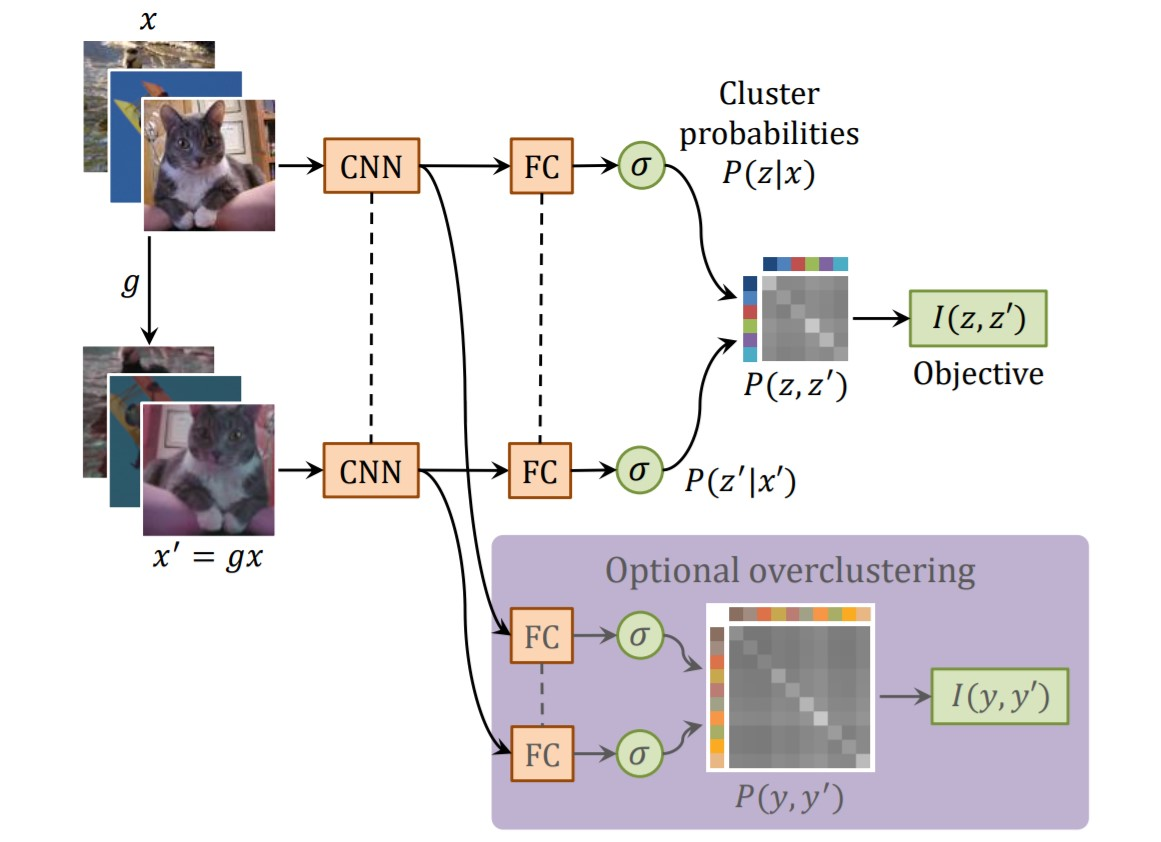
\includegraphics[scale=0.5]{IIC_scheme.jpg}
        \caption{IIC для кластеризации изображений. 
        Пунктирные линии означают общие параметры, $g$~--- случайная аугментация, 
        $I$~--- взаимная информация.\label{fig:iic_scheme}}
    \end{figure}

    Чтобы применить IIC к задаче сегментации, достаточно внести две модификации.
    Во-первых, кластеризация применяется к участкам изображения, размер которых определяется рецептивным полем нейронной сети для каждого пикселя.
    Во-вторых, следует учесть локальную пространственную инвариантность.
    Проще говоря, близлежащие пиксели должны иметь схожие метки.
    А формально~--- пусть $x \in \mathbb{R}^{3 \times H \times W}$ есть RGB-представление изображения,
    $u \in \Omega = \{1, \ldots, H\} \times \{1, \ldots, W\}$ -- позиция пикселя, и $x_u$~--- участок с центром в $u$.
    Мы можем сформировать пару $(x_u, x_{u + t})$, где $t \in \mathbb{Z}^2$~--- небольшие смещения.
    Оптимизируя функцию потерь IIC для такой пары, мы будем добиваться желаемой локальной пространственной инвариантности.
    
    Вообще говоря, мы можем применять одновременно и фотометрические, и геометрические, и пространственные трансформации.
    Надо лишь следить за тем, что мы сравниваем соответствующие участки.
    Если $g$~--- геометрическое преобразование (например, отражение), то $\Phi_u(x)$ соответствует не $\Phi_u(gx)$,
    а $\Phi_{g(u)}(gx)$, так как $x_u$ был отображён в $x_{g(u)}$.
    Однако, пользуясь тем, что $\left[g^{-1} \Phi(g x) \right]_u = \Phi_{g(u)}(g x)$, можно сопоставить все участки одновременно.

    Итого, формулировка задачи для сегментации:
    \begin{gather}
            \max_{\Phi} \frac{1}{T} \sum_{t \in T} \bm{I}(\bm{P}_t),\\
            \bm{P}_t = \frac{1}{n |G| |\Omega|} \sum_{i=1}^{n} \sum_{g \in G} \sum_{u \in \Omega} \Phi_u(x_i) \cdot \left[g^{-1} \Phi(g x) \right]_{u + t}^T \label{eq:joint_distr_iic}
    \end{gather}
    Иными словами, мы максимизируем взаимную информацию между двумя соседними участками, один из которых дополнительно аугментирован,
    причём взаимная информация усредняется по соседям.
    Совместное распределение в уравнении \ref{eq:joint_distr_iic} можно эффективно посчитать, заменяя внутреннюю сумму на операцию свёртки.

    \subsubsection{Результаты}
    Авторы используют датасеты COCO-Stuff и Postdam.
    COCO-Stuff~--- это датасет для сегментации, в котором размечен фон (трава, небо, река и т.д.).
    Авторы используют вариант с 15-ю классами, причём предварительно удаляют изображения, 
    на который доля фоновых пикселей меньше 75\% (видимо, метод хорошо работает именно для сегментации фона, 
    и таким образом ему даётся преимущество).
    COCO-Stuff-3~--- подмножество COCO-Stuff, где всего три класса: небо, земля и растения.
    При оценке качества предсказания для не фоновых пикселей игнорируются.
    
    Postdam содержит 8550 снимков со спутников, из которых 3150 не размечены.
    Изначальная версия содержит 6 классов (дороги и машины, растительность и деревья, строения и беспорядок),
    но авторы также использовали Postdam-3, попарно объединив указанные классы.

    На рисунке \ref{fig:iic_segmentation} можно видеть примеры сегментации с помощью IIC и IIC*.
    Первое~--- полностью unsupervised метод, второй предобучается без меток и с использованием overclusterization, а затем дообучается на небольшом числе изображений 
    (например, в 10 раз меньше, чем нейросеть с учителем).

    На рисунке \ref{fig:iic_results} показаны результаты IIC и предшествующих методов.
    Измеряется метрика accuracy, усреднённая по пикселям (предсказания для пикселей объектов, не принадлежащих рассматриваемым семантическим классам, не учитываются). 
    В случае IIC требуется сопоставить обнаруженные нейросетью кластеры с семантическими классами.
    Это делается с помощью венгерского алгоритма.
    Авторы подчёркивают, что хотя на этом этапе используются метки, это не является частью обучения, 
    а просто гарантирует инвариантность результатов относительно порядка кластеров.
    Для IIC* кластеров больше, чем семантических классов, и набор кластеров может соответствовать одному классу.
    Чтобы найти отображение из кластеров в семантические классы, опять надо использовать метки.
    В этом случае для корректности нужно использовать лишь метки из train, так как в процессе уже существенно используется информация о метках.

    \begin{figure}
        \centering
        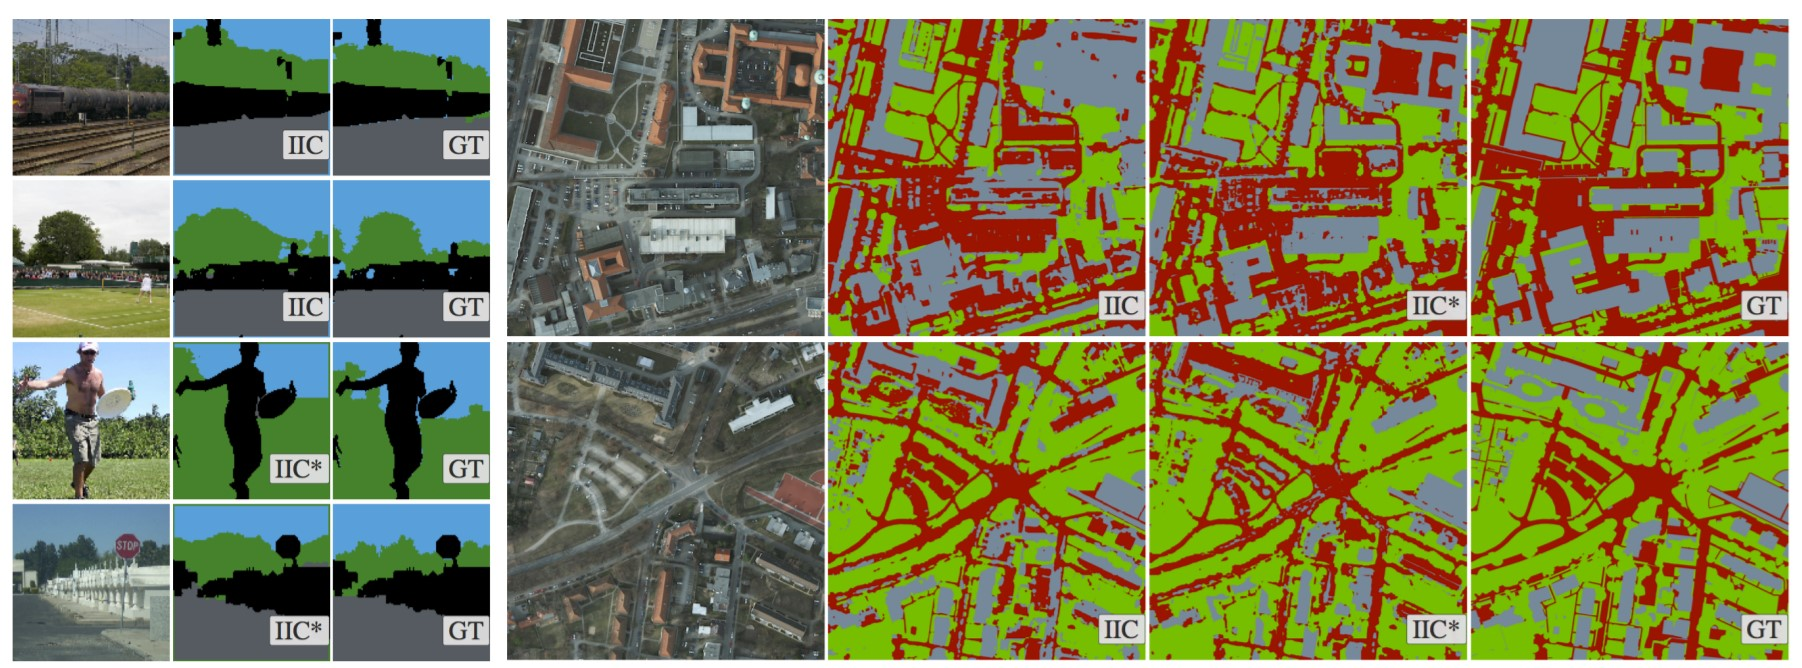
\includegraphics[scale=0.45]{IIC_segmentation.jpg}
        \caption{Слева: COCO-Stuff-3 (объекты отмечены чёрным цветом), справа: Postdam-3.
        Исходные изображения, IIC, IIC*, GT (ground truth -- истинная разметка)\label{fig:iic_segmentation}}
    \end{figure}

    \begin{figure}
        \centering
        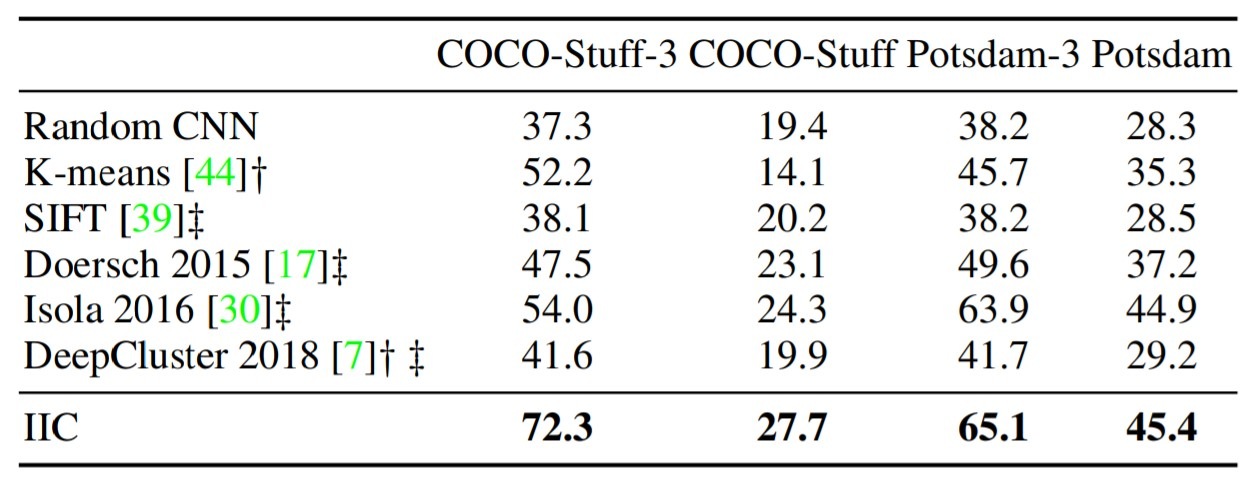
\includegraphics[scale=0.5]{IIC_results.jpg}
        \caption{$\dagger$ -- Методы, основанные на KMeans. 
        $\ddagger$ -- Методы, которые требуют применения KMeans.\label{fig:iic_results}}
    \end{figure}

    \bigskip
    Авторы IIC достигли заметного прогресса в задаче сегментации без учителя и 
    реализовали интересную идею с максимизацией взаимной информации, что позволило избежать вырожденных решений.
    Такой подход, тем не менее, имеет свои недостатки~--- он хорошо работает лишь для фона и плохо справляется с мелкими деталями.

    \FloatBarrier
\subsection{PiCIE}
    \textit{В одно предложение: попеременное обучение признаковых описаний пикселей и кластеризация,
    признаковые описания инвариантны относительно фотометрических и эквивариантны относительно геометрических преобразований.}
    \bigskip

    \begin{figure}
        \centering
        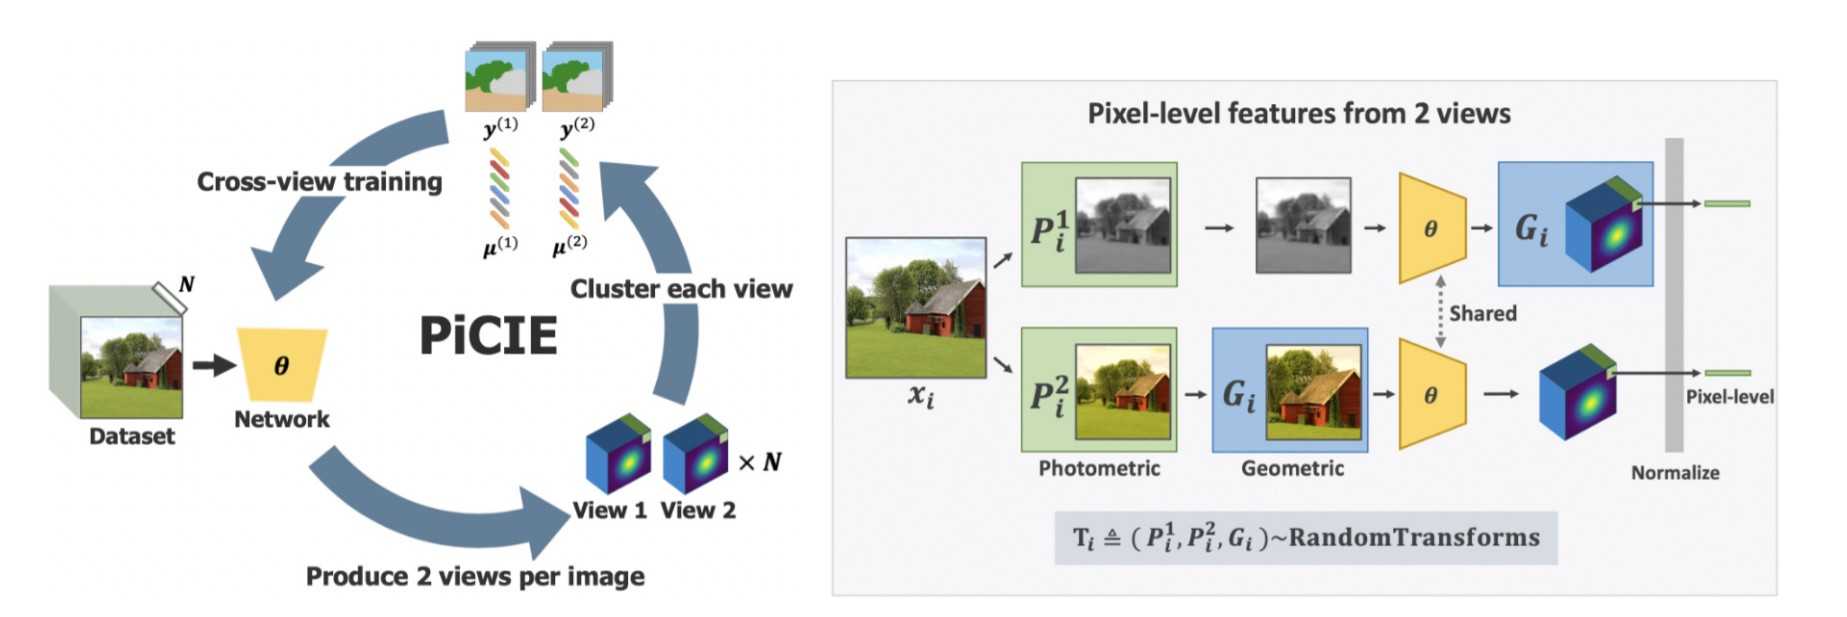
\includegraphics[scale=0.4]{PiCIE_scheme.jpg}
        \caption{Схема PiCIE}
    \end{figure}

    Как уже было сказано, задачу семантической сегментации без учителя можно рассматривать как кластеризацию пикселей.
    В таком случае основная проблема заключается в построении качественного признакового описания.
    К сожалению, здесь возникает проблема курицы и яйца: чтобы получить семантически осмысленные (т.е. разнесённые по кластерам)
    описания пикселей, нужны метки семантических классов, которые мы и пытаемся получить~--- иначе нейросети неоткуда брать сигнал для обучения.

    Решение этой проблемы было предложено в работе Deep Cluster: можно кластеризовать текущие представления 
    и использовать кластера в качестве меток, чтобы обучить новые представления, и повторять этот процесс итеративно.
    Для обучения encoder-а $f$ можно использовать следующую функцию потерь:
    \begin{equation}
        \mathcal{L}_\text{clust} (z_{ip}, y_{ip}, \bm{\mu}) = 
        -\log \left( \frac{e^{-d(z_{ip}, \mu_{y_{ip}})}}{\sum_{l} e^{-d(z_{ip}, \mu_{l})}} \right)
    \end{equation}
    где $d(\cdot, \cdot)$~--- косинусное расстояние, $z_{ip} = f(x_i)_p$ --- признаковое описание $p$-го пикселя $i$-го изображения,
    $y_{ip}$~--- кластер этого пикселя, $\mu_{y_{ip}}$~--- соответствующий центроид, $\bm{\mu} = (\ldots, \mu_l, \ldots)$ --- все центроиды.
    По смыслу это кросс-энтропия, а косинусное расстояние с другим знаком используется в качестве логитов: чем меньше расстояние, тем больше логит и тем выше вероятность правильного кластера.

    В процессе мы можем надеяться получить достаточно компактные кластера пикселей.
    Однако, мы никак не контролируем их семантическую осмысленность.

    Авторы PiCIE предлагают использовать инвариантность относительно фотометрических преобразований 
    и эквивариантность относительно геометрических преобразований. 
    Иными словами, метка пикселя не должна изменяться при небольших колебаниях цвета,
    а если изображение, например, отражено относительно вертикальной оси, то метки также должны быть отражены.
    Более формально, если $P_1, P_2$ --- некоторые фотометрические преобразования, $G$ --- геометрическое преобразование, 
    $f$ --- нейронная сеть, осуществляющая сегментацию, то мы хотим, чтобы
    \begin{equation}    
        f\bigl(G\bigl(P_1(x)\bigr)\bigr) = G\bigl(f\bigl(P_2(x)\bigr)\bigr).
    \end{equation}

    Реализовать такое ограничение не так просто --- псевдоразметка получается кластеризацией имеющихся представлений,
    которые, в свою очередь, зависят от фотометрических преобразований. 
    Как же добиться инвариантности в кластеризации? 

    Пусть $x_i$ --- это $i$-е изображение.
    Для него случайно выбираются фотометрические преобразования $P^{(1)}_i, P^{(2)}_i$.
    Для каждого пикселя каждого изображения мы получаем по два векторных представления
    \begin{gather}
        z_{ip}^{(1)} = f(P^{(1)}_i(x_i))_p\\
        z_{ip}^{(2)} = f(P^{(2)}_i(x_i))_p
    \end{gather}
    Далее производится кластеризация 
    \begin{gather}
        \bm{y}^{(1)}, \bm{\mu}^{(1)} = \argmin_{\bm{y}, \bm{\mu}} \sum_{i, p} \Vert z_{ip}^{(1)} - \mu_{y_{ip}} \Vert^2 \\
        \bm{y}^{(2)}, \bm{\mu}^{(2)} = \argmin_{\bm{y}, \bm{\mu}} \sum_{i, p} \Vert z_{ip}^{(2)} - \mu_{y_{ip}} \Vert^2
    \end{gather}

    Имея два набора центроидов и меток, можно подсчитать значение функции потерь.
    Она состоит из двух слагаемых.
    Во-первых, мы хотим, чтобы пиксели хорошо разделялись на кластера:
    \begin{equation}
        \mathcal{L}_\text{within} = 
        \sum_{i, p} \mathcal{L}_\text{clust}(z^{(1)}_{ip}, y^{(1)}_{ip}, \bm{\mu}^{(1)}) +
        \sum_{i, p} \mathcal{L}_\text{clust}(z^{(2)}_{ip}, y^{(2)}_{ip}, \bm{\mu}^{(2)})
    \end{equation}
    Во-вторых, мы хотим, чтобы кластеризация была инвариантна к фотометрическим преобразованиям, так что появляется ещё одно слагаемое:
    \begin{equation}
        \mathcal{L}_\text{cross} =
        \sum_{i, p} \mathcal{L}_\text{clust}(z^{(1)}_{ip}, y^{(2)}_{ip}, \bm{\mu}^{(2)}) +
        \sum_{i, p} \mathcal{L}_\text{clust}(z^{(2)}_{ip}, y^{(1)}_{ip}, \bm{\mu}^{(1)})
    \end{equation}
    Итоговая функция потерь получается суммированием:
    \begin{equation}
        \mathcal{L}_\text{total} = \mathcal{L}_\text{cross} + \mathcal{L}_\text{within}
    \end{equation}

    Чтобы добиться эквивариантности к геометрическим преобразованиям, достаточно положить в вышеописанной схеме
    \begin{gather}
        z_{ip}^{(1)} = f\bigl(G(P^{(1)}_i(x_i))\bigr)_p\\
        z_{ip}^{(2)} = G\bigl(f(P^{(2)}_i(x_i))_p\bigr)
    \end{gather}
    где $G$ --- случайно выбранная геометрическая трансформация (отражение, приближение и т.д.).

    Для стабилизации обучения оказалось полезно одновременно оптимизировать эту же функцию потерь с большим числом кластеров.
    Обычно при использовании нескольких функций потерь коэффициенты перед ними трактуются как гиперпараметры.
    Однако, в полностью unsupervised-режиме подбор гиперпараметров невозможен, так как за неимением меток мы не можем оценить качество разных гиперпараметров.
    Авторы балансируют вклад основного и вспомогательного лосса следующим образом:
    \begin{equation}
        \mathcal{L} = \frac{\log K_2}{\log K_1 + \log K_2} \mathcal{L}_{K_1} + \frac{\log K_1}{\log K_1 + \log K_2} \mathcal{L}_{K_2} 
    \end{equation}
    Интуиция~--- кросс-энтропия логарифмически зависит от числа кластеров, 
    так что следует уменьшить вклад дополнительной функции потерь, дабы она не подавляла основную.

    На рисунке \ref{fig:picie_pictures} можно видеть примеры сегментации в сравнении с предыдущим наилучшим методом
    и с сегментацией с учителем. В таблицах 2, 3, 4 на рисунке \ref{fig:picie_results} указаны метрики Accuracy и mean IoU (среднее IoU по всем классам).
    Стоит отметить, что PiCIE значительно лучше работает для категории Things.
    Авторы предполагают, что это следствие эквивариантности к геометрическим преобразованиям.

    \begin{figure}
        \centering
        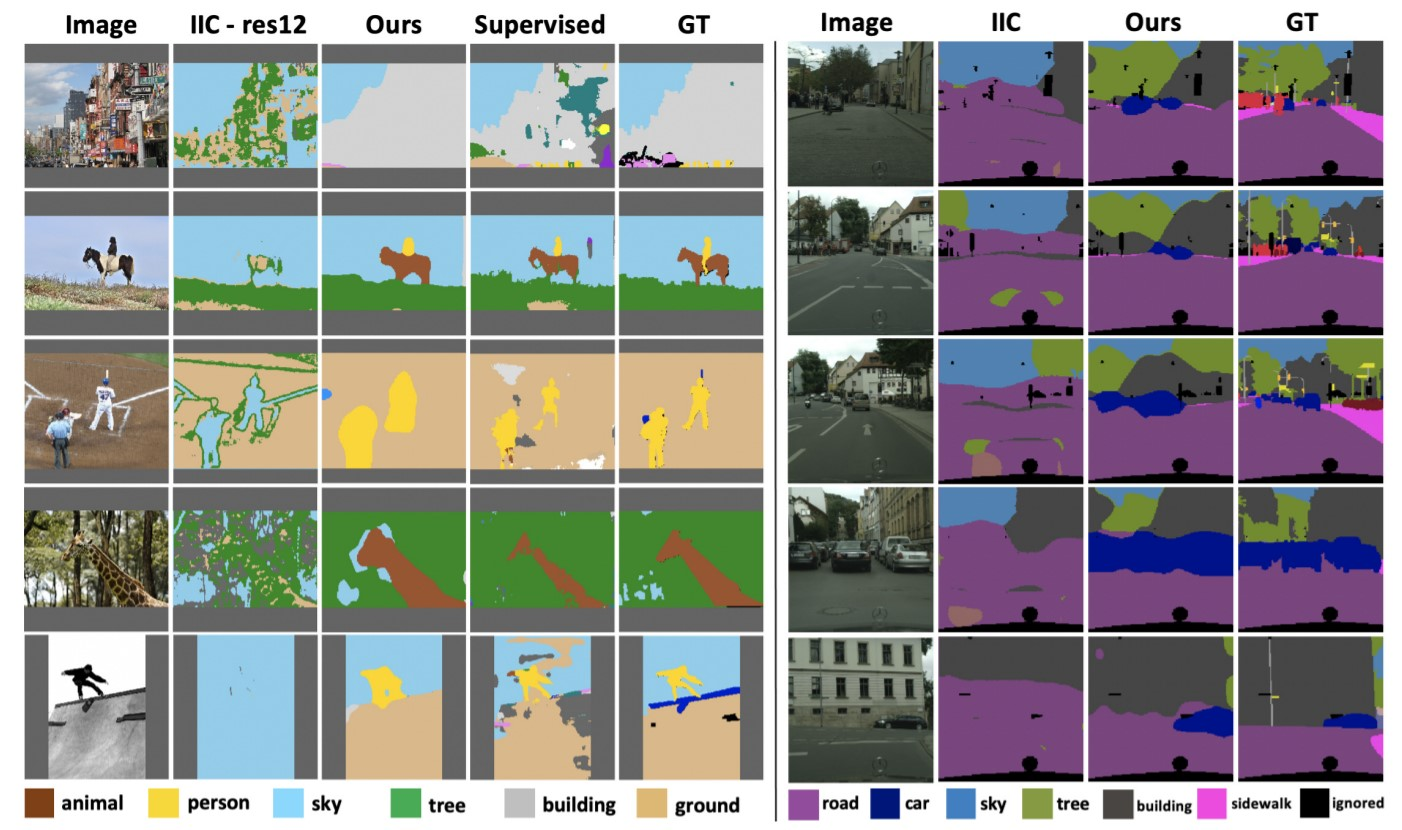
\includegraphics[scale=0.5]{PiCIE_pictures.jpg}
        \caption{Результаты на CoCo-All (слева) и Cityscapes (справа). 
        Сравнение с Infomation Invariant Clustering (IIC, IIC-res12) 
        и с сегментацией с учителем (supervised) \label{fig:picie_pictures}}
    \end{figure}

    \begin{figure}
        \centering
        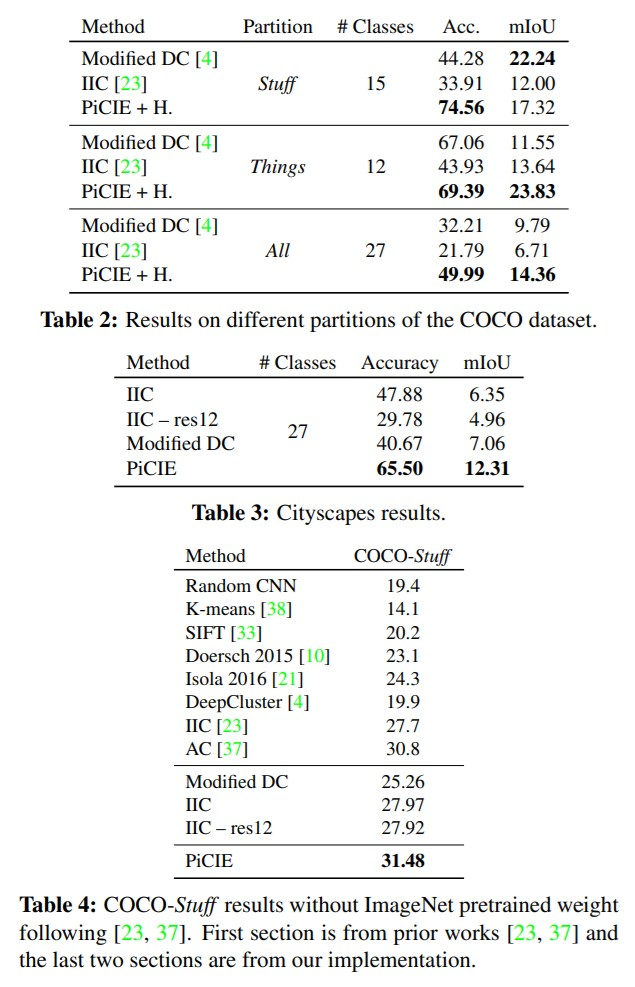
\includegraphics[scale=1.0]{PiCIE_results_234.jpg}
        \caption{Результаты PiCIE \label{fig:picie_results}}
    \end{figure}

    Интересно также взглянуть на то, какой прирост даёт каждая компонента алгоритма: это отражено в таблицах 5 и 6 на рисунке \ref{fig:picie_ablation}.
    Например, использование одного набора центроидов только с геометрическими преобразованиями, 
    замена $\mathcal{L}_\text{cross}$ на MSE между $z^{(1)}, z^{(2)}$ и отсутствие балансирования функций потерь ведут к снижению качества.

    \begin{figure}
        \centering
        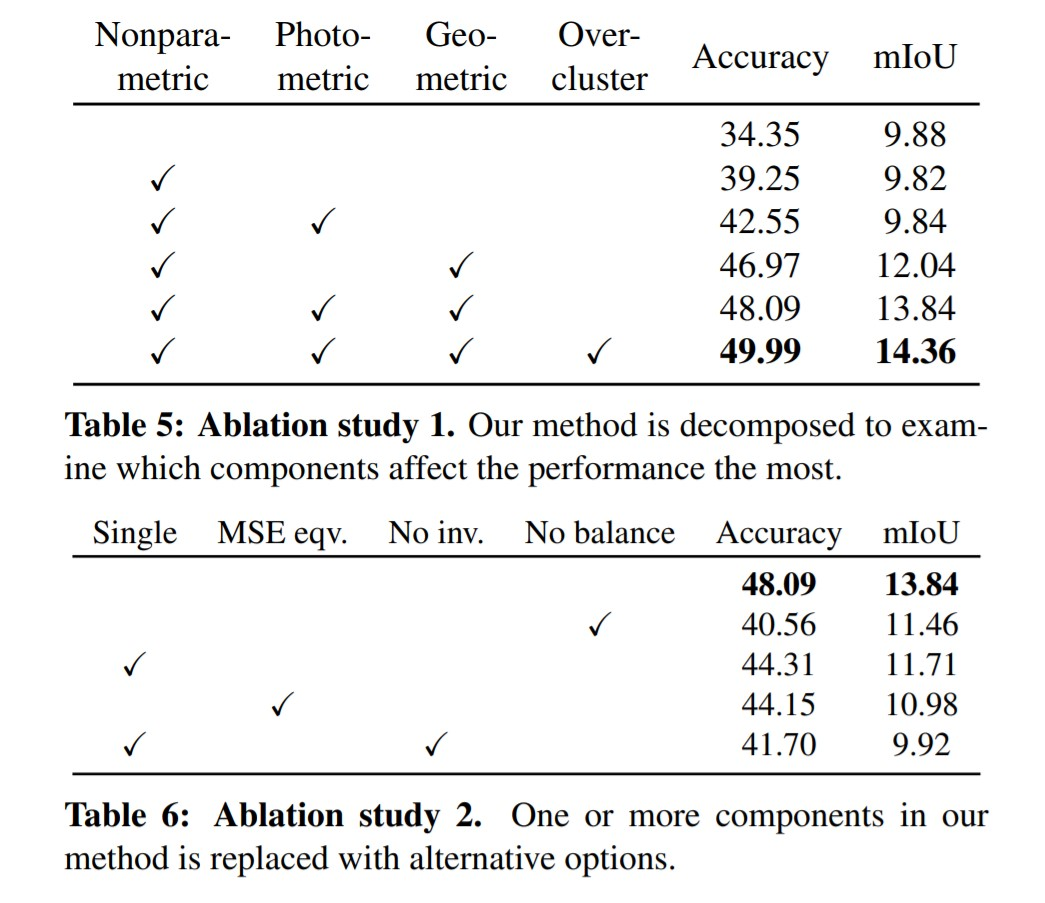
\includegraphics[scale=0.7]{PiCIE_ablation.jpg}
        \caption{Важность компонент \label{fig:picie_ablation}}
    \end{figure}

    \begin{figure}
        \centering
        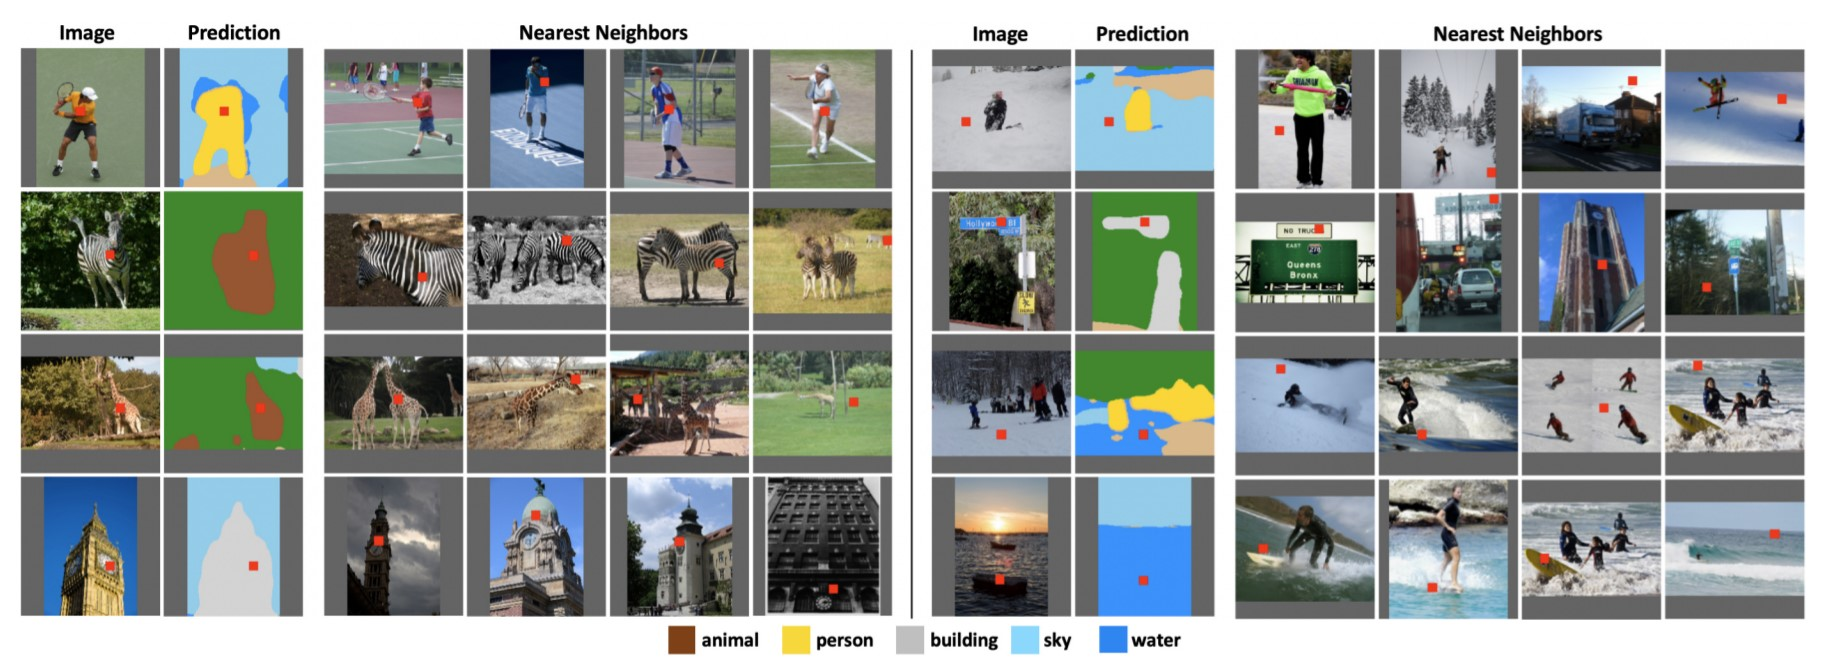
\includegraphics[scale=0.45]{PiCIE_neighbours.jpg}
        \caption{Ближайшие соседи выделенных красным пикселей на других изображениях. \label{fig:picie_neighbours}}
    \end{figure}

    Имея семантически осмысленное латентное представление пикселя, мы получаем возможность искать ближайших к нему соседей на других изображениях.
    На рисунке \ref{fig:picie_neighbours} можно видеть примеры. Слева показаны правильно найденные соседи (принадлежащие тому же семантическому классу --- зебра, жираф, здание).
    Справа приведены случаи, где семантический класс ближайшего соседа оказался другим.
    Стоит отметить, что ошибки объяснимы --- например, в первом ряду нейросеть спутала снег и облака, так как они довольно похожи.

    \FloatBarrier

\subsection{DINO}
    \textit{В одно предложение --- внимание CLS-токена в DINO хорошо выделяет объекты.}
    \bigskip

    Долгое время в компьютерном зрении доминирующую позицию занимали свёрточные нейронные сети.
    При этом в обработке естественного языка с 2017 года основной архитектурой является трансформер.
    Естественно, люди пытались применить их к задачам распознавания изображений, однако долгое время результаты были достаточно скромными ---
    при обучении на Imagenet без сильной регуляризации трансформеры выдавали точность на несколько процентов ниже, чем ResNet с таким же числом параметров. 
    Но в 2021 году была опубликована статья <<An Image is Worth 16x16 Words: Transformers for Image Recognition at Scale>>,
    в которой было показано, что трансформеры, предобученные на очень больших объёмах данных ($\sim 300$ млн изображений), не уступают CNN.
    Это дало сильный толчок развитию исследований в этой области.

    Очевидно, требование большого количества размеченных данных для обучения~--- это существенный минус.
    В обработке естественного языка нашли изящный выход: оказывается, можно придумать задачу, для которой разметку 
    можно получить автоматически и для любого количества данных. Такой задачей является, например, Masked Langauge Modeling:
    нейросети на вход подаётся текст, причём некоторые слова заменяются на пропуск (маскируются), и требуется предсказать, что же пропущено.
    %Чтобы создать датасет для такой задачи, достаточно, например, взять все тексты из Википедии и маскировать в них случайные слова.
    %При этом мы знаем, что именно мы маскировали, и можем проверить, правильно ли сработала нейросеть.
    
    Задачи, для которых разметку можно получить автоматически из самих данных, относят к области Self-Supervised Learning.
    С приходом трансформеров в компьютерное зрение она стала значительно популярнее, так как позволяет избавиться от нужды в титанических размеченных датасетах.
    Авторы статьи <<Emerging Properties in Self-Supervised Vision Transformers>> предлагают новый метод self-supervised обучения для vision transformer-а,
    который не только показывает хорошие результаты на нескольких задачах, но и ведёт к возникновению некоторых интересных свойств.
    
    \subsubsection{Обучение}
    Метод обучения схематично изображён на рисунке \ref{fig:dino_scheme}.
    На вход студенту и учителю подаются две случайные трансформации входного изображения.
    Студент и учитель имеют одинаковые архитектуры, но разные наборы параметров.
    На выходе получаем некоторое векторное представление для исходных изображений.
    К ним применяется операция softmax, а затем между ними считается кросс-энтропия.
    Важная особенность: вектор от учителя перед взятием softmax-а центрируется,
    а потом все элементы делятся на маленькое число.
    Если оставить только центрирование, то учитель будет тяготеть к равномерному распределению в ответ на любое изображение;
    если оставить только масштабирование, то учитель станет предсказывать распределение, вырожденное в одной точке,
    так что для балансирования надо использовать и то, и другое.
    
    \begin{figure}
        \centering
        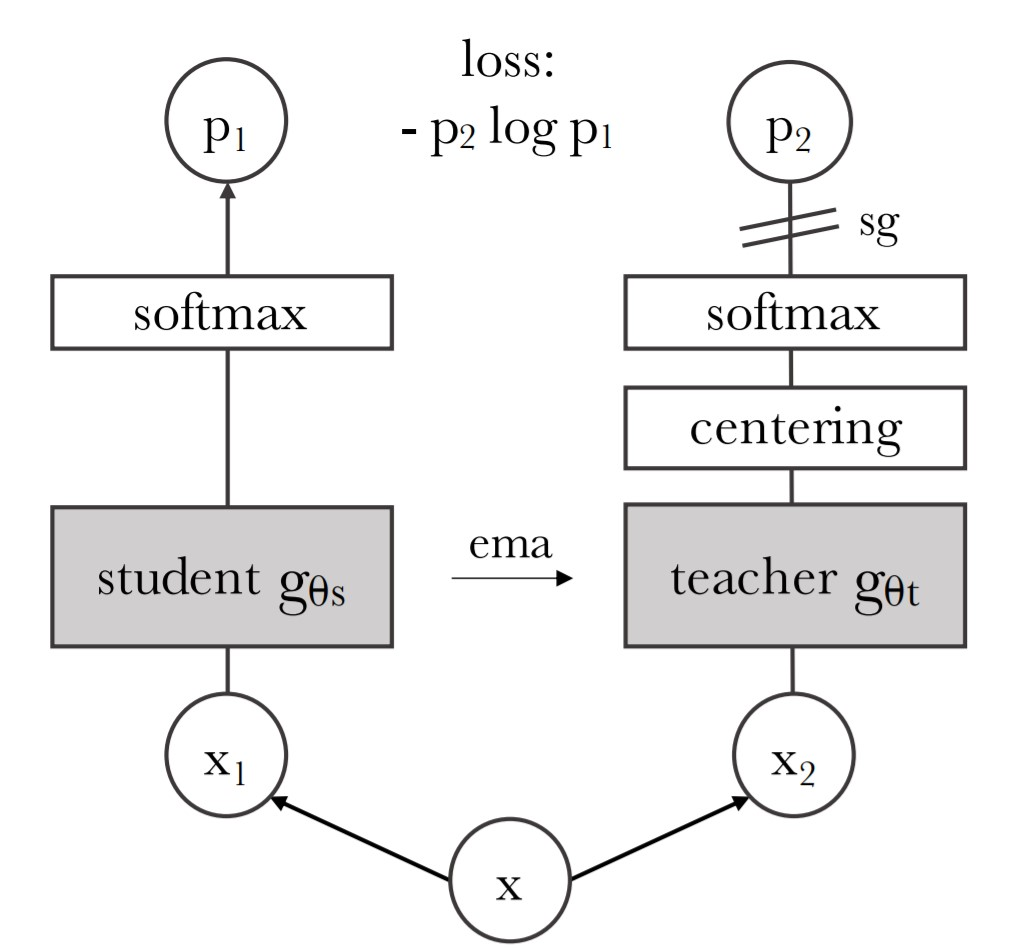
\includegraphics[scale=0.4]{DINO_scheme.jpg}
        \caption{Схема обучения DINO\label{fig:dino_scheme}}
    \end{figure}
    
    Веса учителя обновляются не градиентным спуском (sg на рисунке означает stop-gradient), а считаются как экспоненциальное среднее весов студента.
    Т.е.
    \begin{equation}
        \theta_t^{(k+1)} = \lambda \theta_t^{(k)} + (1 - \lambda) \theta_s^{(k + 1)}
    \end{equation}
    Усреднение весов здесь имеет смысл ансамблирования моделей.
    На протяжении всего обучения учитель производит более качественные эмбеддинги изображений, тем самым направляя обучение студента.

    Центрирующее слагаемое $c$ также обновляется с помощью экспоненциального сглаживания:
    \begin{equation}
        c^{(k + 1)} = m c^{(k)} + (1 - m) \frac{1}{B} \sum_{i=1}^B g_{\theta_t} (x_i)
    \end{equation}

    \subsubsection{Результаты}
    На рисунке \ref{fig:dino_video_segm} можно видеть численные результаты.
    Оценивание проведено для сегментации видео.
    Авторы говорят, что использовали метод ближайших соседей между рядом стоящими кадрами.
    \textit{Не очень понятно, как именно произведена сегментация,} однако результаты превосходят многие сильные бейзлайны.

    На рисунке \ref{fig:dino_cherry} показаны примеры сегментации с использование карт внимания от разных голов токена CLS с последнего слоя трансформера.
    Маску образуют все патчи, которым присвоен вес больше некоторого порога, причём порог выбирается так, чтобы сохранить 60\% от суммы всех весов.

    Исследуя важность различных компонент обучения, авторы установили, что важно использовать аугментацию multicrop.
    Она заключается в том, что из изображения вырезаются небольшие кусочки, которые подаются студенту, а учитель видит либо 
    всё изображение целиком, либо б\'{о}льший кусок.
    Студент должен предсказать такой же эмбеддинг, как и учитель, поэтому ему приходится восстанавливать семантику изображения по небольшому участку.
    Вероятно, поэтому он концентрирует своё внимание на объектах или его частях, потому что именно в них содержится основная информация на изображении.
    Можно предположить, что задача, решаемая DINO при предобучении, несёт более полезный сигнал для сегментации.
    В самом деле, на рисунке \ref{fig:dino_cherry_2} авторы сравнивают нейросеть, обученную с помощью DINO, с нейросетью, предобученной с помощью  supervised learning.
    У последней не возникает эффекта сегментации. 

    \begin{figure}
        \centering
        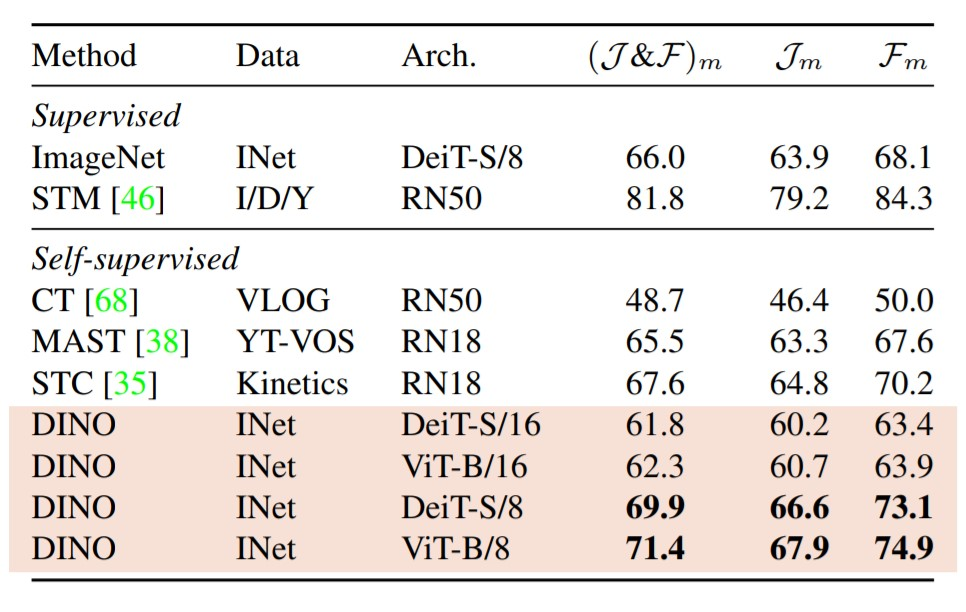
\includegraphics[scale=0.4]{DINO_video_segm.jpg}
        \caption{DAVIS 2017 Сегментация объектов на видео.
        $\mathcal{J}_m$ -- это mIoU, $\mathcal{F}_m$ -- метрика, оценивающая точность предсказания границ сегментации.
        \label{fig:dino_video_segm}}
    \end{figure}

    \begin{figure}
        \centering
        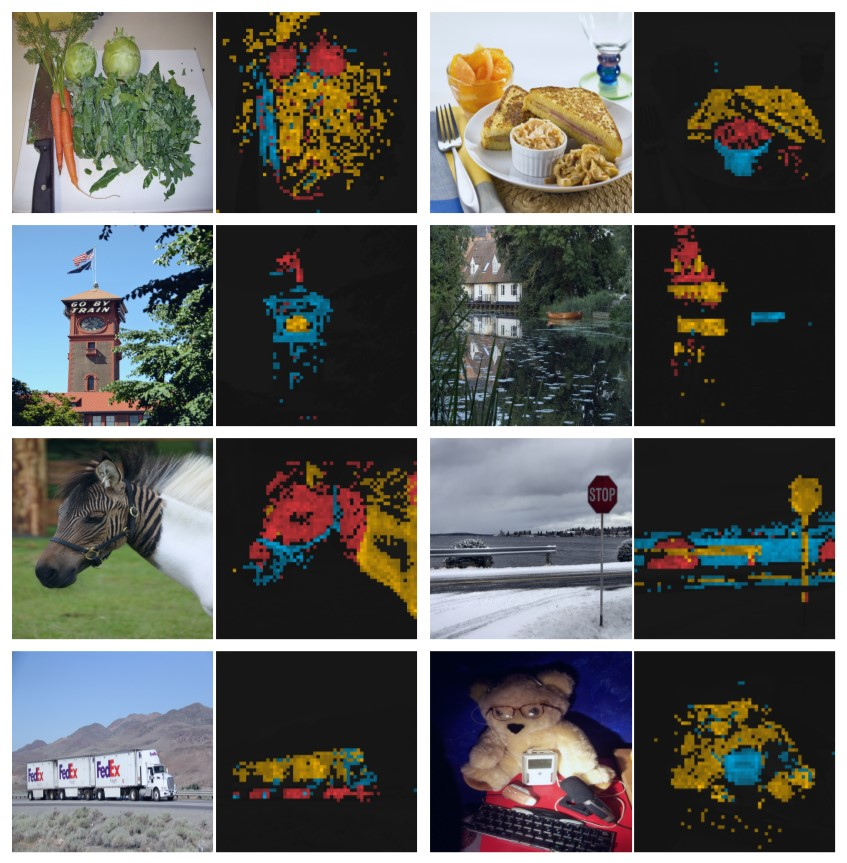
\includegraphics[scale=0.5]{DINO_cherry.jpg}
        \caption{Карты внимания разных голов для токена CLS.
        Разные головы, показанные разным цветом, фокусируются на разных объектах или их частях.
        \label{fig:dino_cherry}}
    \end{figure}

    \begin{figure}
        \centering
        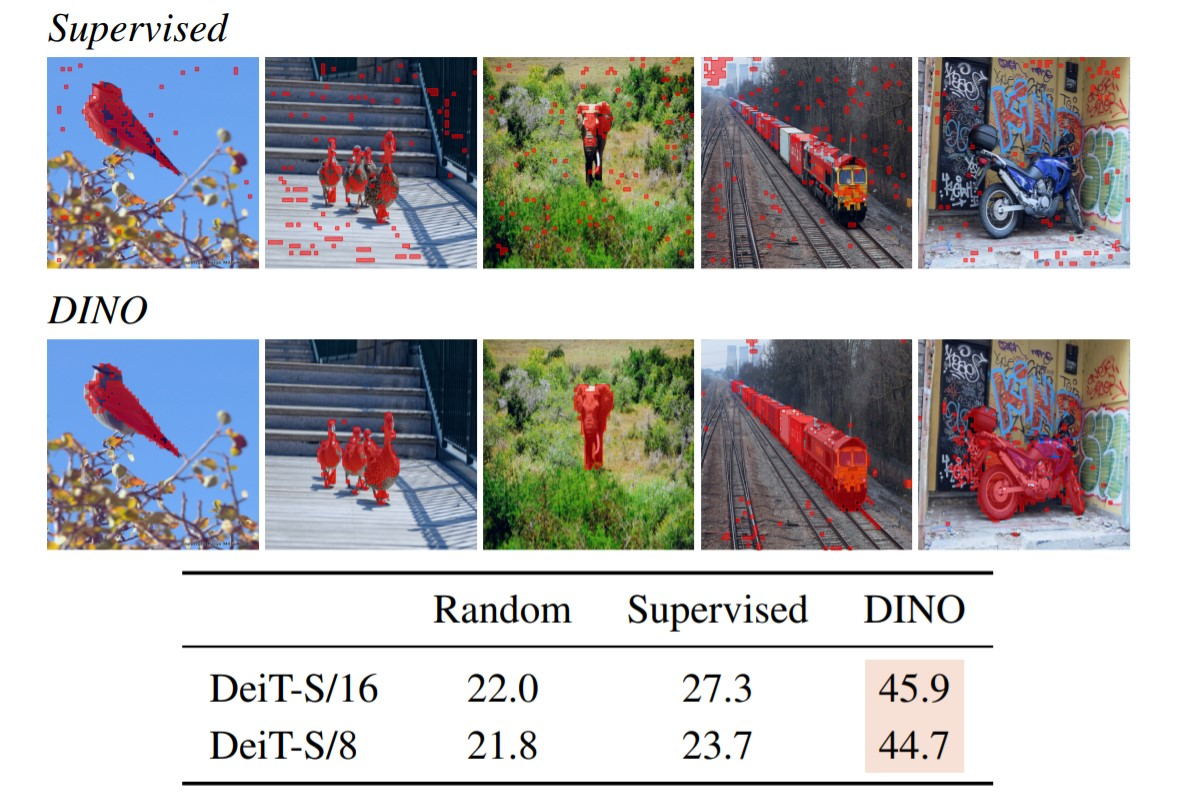
\includegraphics[scale=0.5]{DINO_cherry_2.jpg}
        \caption{Сегментация с помощью карт внимания для DINO и supervised-модели.
        Показана лучшая голова для обоих моделей.
        Таблица сравнивает коэффициент Жаккара между правильной сегментаций 
        и валидационными изображениями в PASCAL VOC12.
        \label{fig:dino_cherry_2}}
    \end{figure}

    \FloatBarrier

\subsection{Stego}
    \textit{В одно предложение --- дистилляция признаковых описаний пикселей от DINO с сохранением корреляции признаковых описаний.}
    \bigskip

    Как стало известно в последние годы, промежуточные представления в нейронных сетях могут быть хорошим признаковым описанием или инымы способами нести полезный сигнал.
    Например, в статье RAFT: Recurrent All-Pairs Field Transforms for Optical Flow удаётся использовать четырёхмерные тензоры корреляций между картами активаций.
    Они определяются следующим образом: пусть $A \in \mathbb{R}^{C H W}$, $B \in \mathbb{R}^{C I J}$~--- признаковые тензоры двух изображений,
    где $C$ отвечает за размерность представления одного пикселя, а $(H, W), (I, J)$ отвечают за размеры изображений.
    Тогда тензор корреляций (или тензор соответствий признаков) $F$ есть
    \begin{equation}
        F \in \mathbb{R}^{H W I J}, \quad F_{hwij} = \sum_{c} \frac{A_{chw}}{\vert A_{hw}\vert} \frac{B_{cij}}{\vert B_{ij}\vert}
    \end{equation}
    Его элементы~--- это косинусное расстояние между признаковым описанием пикселя на позиции $(h, w)$ с первого изображения и на позиции $(i, j)$ со второго. 
    Если оно мало, то указанные пиксели схожи в признаковом пространстве.
    На рисунке \ref{fig:stego_correlation} на Figure 2 можно видеть, как три избранных точки на изображении соотносятся с остальными точками этого же изображения, а также на ближайших соседях выбранного изображения. 
    Признаковое описание здесь получено с помощью DINO (self-\textbf{di}stillation with \textbf{no} labels).

    \begin{figure}
        \centering
        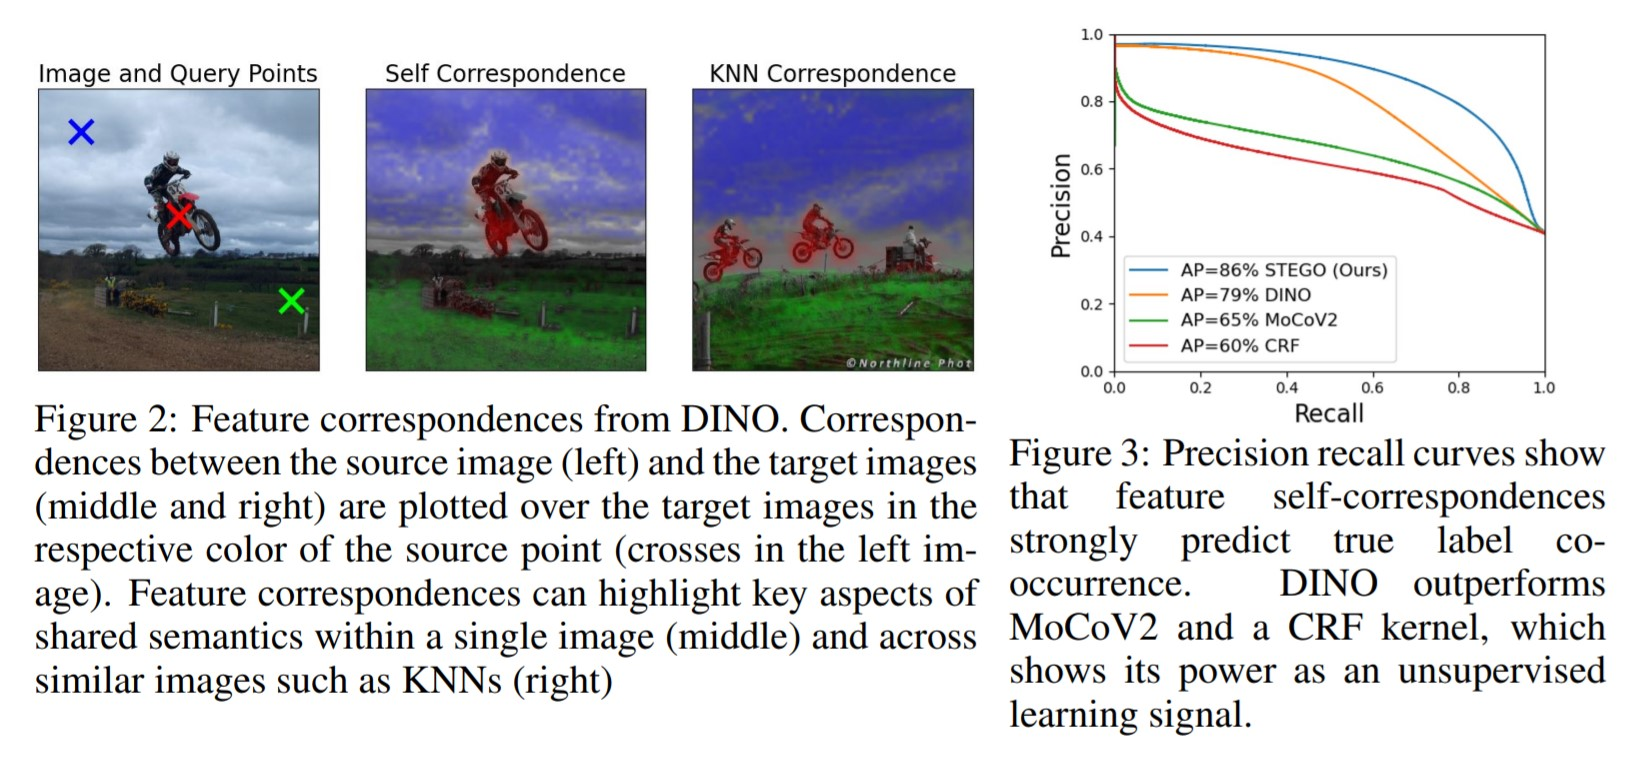
\includegraphics[scale=0.5]{Stego_correlation.jpg}
        \caption{Соответствия между пикселями при использовании DINO.\label{fig:stego_correlation}}
    \end{figure}

    Оказывается, соответствия пикселей сильно скоррелированы с соответствиями меток при семантической сегментации.
    Если использовать косинусное сходство между пикселями как логит для предсказания того, совпадают ли метки этих пикселей,
    то беря признаковое описание от DINO без каких-либо изменений, можно получить recall 50\% при precision 90\%.
    Иными словами, мы найдём найдём половину всех пар пикселей с совпадающими метками, при этом лишь 10\% предсказаний будут ложно-положительными.
    Учитывая то, что DINO обучается без разметки и на задачу, слабо связанную с сегментацией, это довольно впечатляющий результат.
    На Figure 3 можно увидеть precision-recall кривую для задачи нахождения пар пикселей с совпадающими метками для нескольких методов.

    Убедившись, что соответствия признаковых описаний пикселей хорошо коррелируют с совпадением семантических меток, авторы решили обучить нейронную сеть, 
    которая бы преобразовывала признаковое описание, полученное от DINO или другого encoder-а, в новое промежуточное представление,
    причём так, чтобы сохранить соответствие между пикселями.

    Более формально, пусть отображение $\mathcal{N}\colon \mathbb{R}^{C' H' W'} \mapsto \mathbb{R}^{C H W}$ --- это исходный encoder,
    который отображает изображение с $C'$ каналами размером $(H', W')$ в признаковый тензор с $C$ каналами размера $(H, W)$.
    Мы хотим обучить легковесную <<голову>> $\mathcal{S}\colon \mathbb{R}^{C H W} \mapsto \mathbb{R}^{K H W}$, 
    которая отображает пиксели из исходного пространства в новое, причём $K < C$.
    Цель $\mathcal{S}$~--- описать такое нелинейное преобразование, чтобы в пространстве $\mathbb{R}^{K H W}$
    образовывались плотные кластера и усиливались паттерны, присутствующие в тензоре корреляций исходных признаков.

    Пусть $x, y$~--- изображения. Рассмотрим тензоры исходных признаков
    \begin{equation}
        f = \mathcal{N}(x) \in \mathbb{R}^{CHW}, \; g = \mathcal{N}(y) \in \mathbb{R}^{CIJ}
    \end{equation}
    и признаков после преобразования $\mathcal{S}$
    \begin{equation}
        s = \mathcal{S}(f) \in \mathbb{R}^{KHW}, \; t = \mathcal{S}(g) \in \mathbb{R}^{KIJ}
    \end{equation}
    Обозначим $F, S$ ---  тензоры корреляций $(f, g), (s, t)$ соответственно.
    Если значение $F_{hwij}$ велико, это значит, что пиксель на позиции $(h,w)$ в изображении $x$ похож на пиксель на позиции $(i,j)$ в изображении $y$.
    Тогда мы хотим, чтобы $S_{hwij}$ также было велико.
    Этого можно добиться, используя следующую функцию потерь:
    \begin{equation}
        \mathcal{L}_\text{simple-corr}(x, y, b) = -\sum_{h, w, i, j} (F_{hwij} - b) S_{hwij}
    \end{equation}
    Параметр $b$ интерпретируется как постоянное <<негативное давление>>, которое не даёт решению сколлапсировать.
    По смыслу, такая фукция потерь заставляет $S_{hwij}$ расти, если $(F_{hwij} - b) > 0$ (т.е. пиксели достаточно схожи), и убывать иначе.

    Эта версия функции потерь оказалось нестабильной.
    Авторы предполагают, что виной тому коллинеарность получающихся представлений.
    Кроме того, для маленьких объектов часто $(F_{hwij} - b) < 0$, и вместо того чтобы выравнивать признаковые описания пикселей этого объекта, сеть делает противоположное.
    Потому предлагается использовать следующую версию:
    \begin{gather}
        \hat{F}_{hwij} = F_{hwij} - \frac{1}{IJ} \sum_{k, m} F_{hwkm} \\
        \mathcal{L}_\text{corr}(x, y, b) = -\sum_{h, w, i, j} (\hat{F}_{hwij} - b) \max(S_{hwij}, 0)
    \end{gather}
    Центрирование корреляции помогает для небольших объектов, а обрезка $S_{hwij}$ в нуле заставляет делать представления отличающихся пикселей ортогональными.

    Данная функция потерь применяется трижды~--- для сравнения изображения с самим собой, с его ближайшими соседями и с случайными изображениями.
    Сравнение с собой и с ближайшими соседями даёт в основном положительный сигнал, а последнее~--- отрицательный.
    Итого получаем 
    \begin{equation}
        \mathcal{L} = \lambda_\text{self} \mathcal{L}_\text{corr}(x, x, b_\text{self}) + 
        \lambda_\text{knn} \mathcal{L}_\text{corr}(x, x_\text{knn}, b_\text{knn}) +
        \lambda_\text{rand} \mathcal{L}_\text{corr}(x, x_\text{rand}, b_\text{rand}) 
    \end{equation}
    Параметры $b$ были подобраны так, чтобы средняя схожесть признаков с ближайшими соседями была $\approx 0.3$, а со случайными изображениями $\approx 0.0$.
    Соотношение между коэффициентами: $\lambda_\text{self} \approx \lambda_\text{rand} \approx 2 \lambda_\text{knn}$ (подобрано эмпирически).

    Чтобы хорошо сегментировать маленькие объекты, авторы вырезают из каждого изображения по 5 локальных участков и при дальнейшем обучении ищут ближайших соседей именно среди этих участков.
    Наконец, чтобы получить метки, надо кластеризовать признаковые описания пикселей, полученные с помощью $\mathcal{S}$.
    Авторы также используют Conditional Random Field, чтобы подправить сегментацию в соответствии с границами на изображении.
    Итоговая схема обучения представлена на рисунке \ref{fig:stego_scheme}.

    \begin{figure}
        \centering
        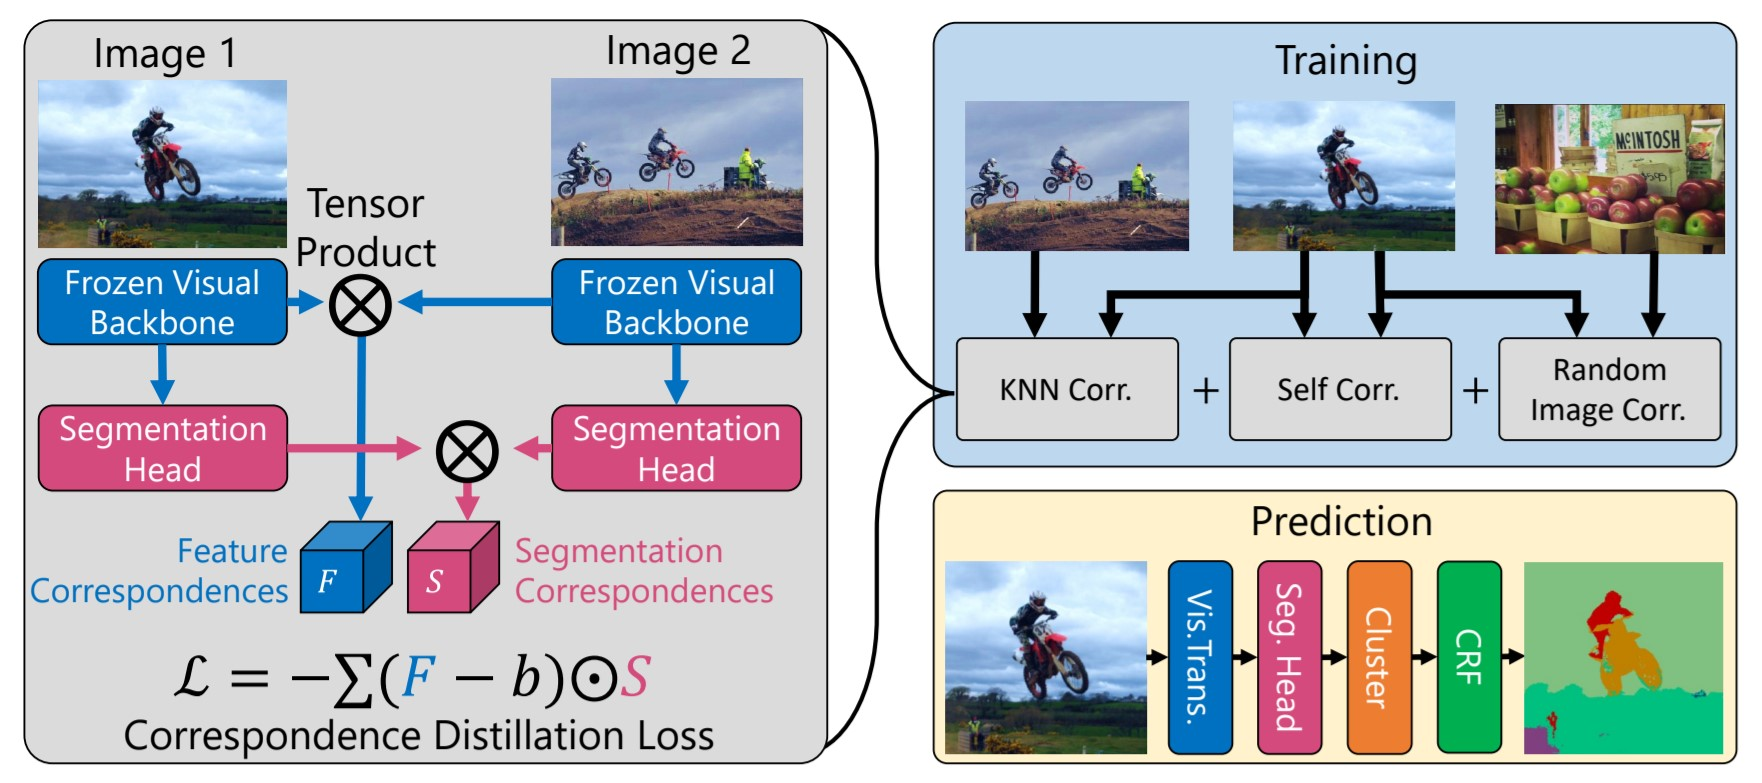
\includegraphics[scale=0.4]{Stego_scheme.jpg}
        \caption{Схема обучения Stego. Серые прямоугольники обозначают функцию потерь.\label{fig:stego_scheme}}
    \end{figure}

    
    Результаты можно видеть на рисунках \ref{fig:stego_results}, \ref{fig:stego_confusion_matrix}.
    \begin{figure}
        \centering
        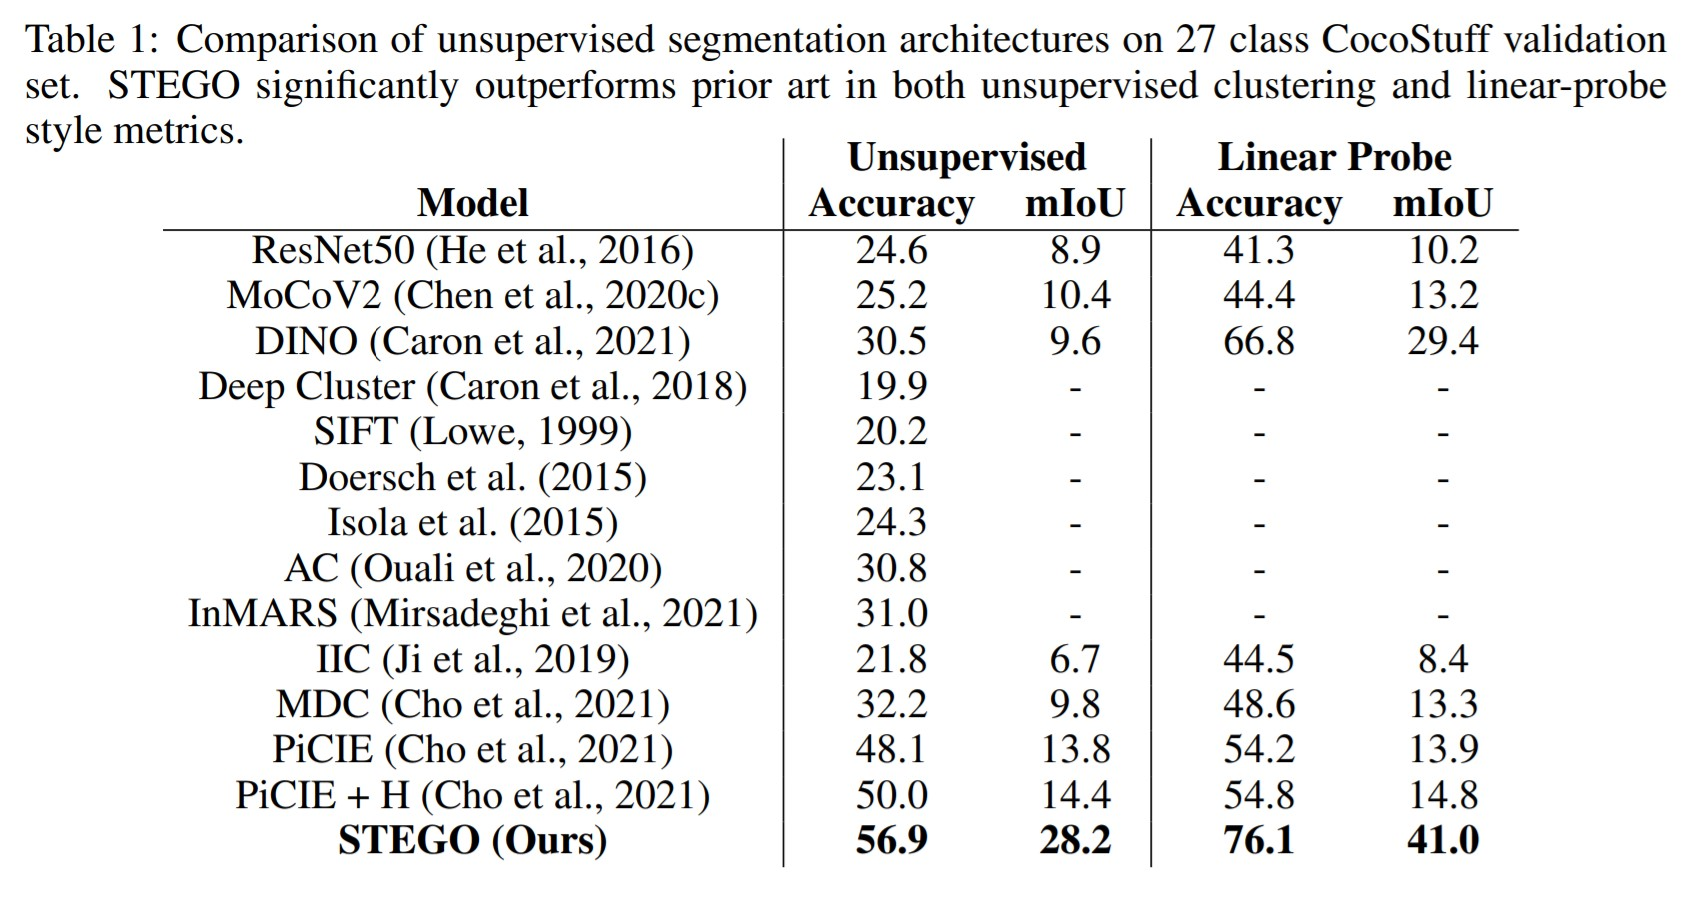
\includegraphics[scale=0.4]{Stego_results.jpg}
        \caption{Результаты на CoCo Stuff\label{fig:stego_results}}
    \end{figure}

    \begin{figure}
        \centering
        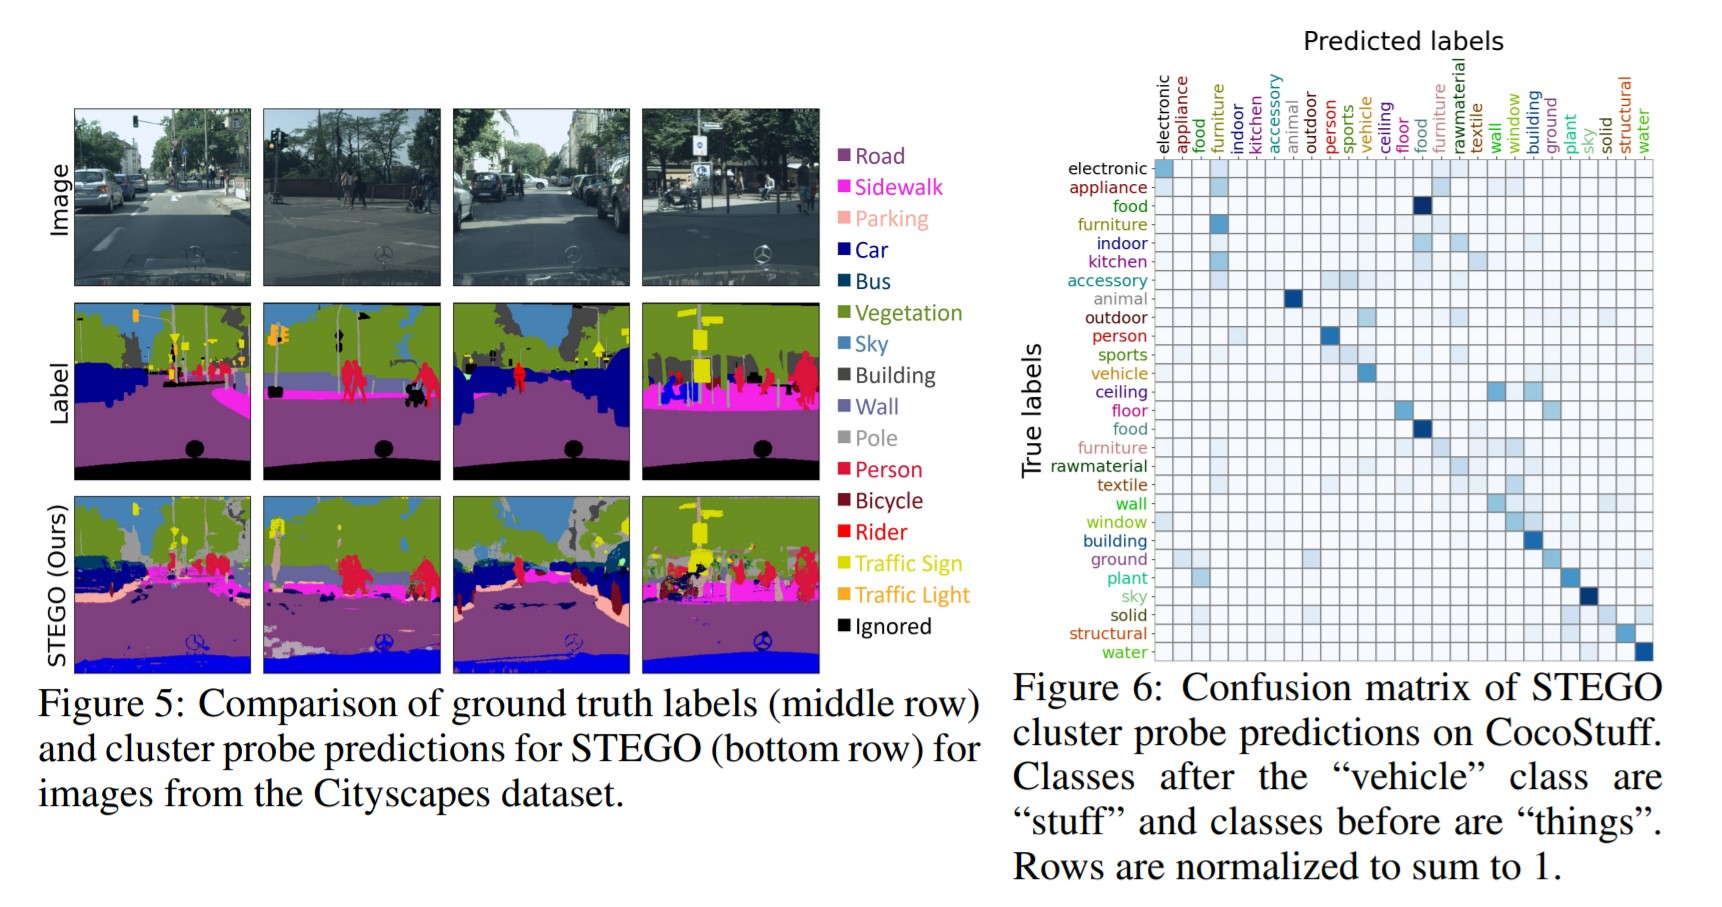
\includegraphics[scale=0.4]{Stego_confusion_matrix.jpg}
        \caption{Пример сегментации. Матрица ошибок\label{fig:stego_confusion_matrix}}
    \end{figure}

    \FloatBarrier
\subsection{Ours}
    \textit{В одно предложение: (пока) замена Selective Search в DETReg на генерацию синтетического датасета с помощью CutMix.}

    Пока удалось проверить только качество детекции.
    \begin{table}
        \caption{Дообучение на детекцию на PASCAL VOC\label{table:ours}}
        \begin{center}
            \begin{tabular}{c c c c}
                \hline
                Метод & detection mAP50 & detection mAP75 & detection mAP \\
                \hline \hline
                DETReg & \textbf{63.5} & 83.3 & 70.3 \\
                Ours & \textbf{63.5} & \textbf{83.8} & \textbf{70.9} \\
                \hline
            \end{tabular}
        \end{center}
    \end{table}